\chapter{无序与局域化}

理想晶体是高度有序的,但是实际的固体多少具有一些无序性。使用格点

\section{Anderson局域化}\label{sec:anderson-localization}

\subsection{固体中的无序}

本节将介绍一种现象:当固体中出现无序,即平移对称性破缺时,电子会倾向于留在原地而不发生长距离跃迁。
这种现象称为\concept{Anderson局域化}。无序可以来自掺杂,也可以来自离子实实际上并没有构成晶体这一事实。

例如可以写出这样的一个带有格点无序的紧束缚模型:
\begin{equation}
    {H} = - t \sum_{\pair{\vb*{i}, \vb*{j}}} ({c}_{\vb*{i}}^\dagger {c}_{\vb*{j}} + \text{h.c.}) + \sum_{\vb*{i}} \epsilon_{\vb*{i}} {c}_{\vb*{i}}^\dagger {c}_{\vb*{i}},
    \label{eq:tight-binding-with-disorder}
\end{equation}
其中$\epsilon_{\vb*{i}}$是一个随机变量,它基本上就是一个在空间各点不一样的“化学势”,让一些地方比另一些地方更能够留住电子。
接下来考虑这样的$\epsilon_{\vb*{i}}$的分布特例:
\begin{equation}
    \overline{\epsilon_{\vb*{i}}} = 0, \quad \overline{\epsilon_{\vb*{i}} \epsilon_{\vb*{j}}} = \delta_{\vb*{i} \vb*{j}} W^2 , \quad W^2 \neq 0.
\end{equation}
这样,$W/t$就表征了无序的大小。
这里我们使用$\overline{\cdots}$表示对杂质的构型的平均,而用$\expval*{\cdots}$表示给定杂质的构型之后做量子力学的平均。
如果$\epsilon_{\vb*{i}}$的分布服从高斯分布,对$\overline{\cdots}$同样有Wick定理成立,这将为后面的费曼图计算提供很大的方便。

在$W/t=0$时就得到一个普通的能带,而如果$W/t \gg 1$,即无序很强,则体系的哈密顿量近似为
\[
    {H} = \sum_{\vb*{i}} \epsilon_{\vb*{i}} {c}_{\vb*{i}}^\dagger {c}_{\vb*{i}},
\]
这个哈密顿量在以瓦尼尔波函数为基底的表象下是对角化的,这样电子倾向于固定在原地,即出现局域化。另一方面,完全没有随机扰动时,电子可以自由地移动。
这意味着随着$W/t$的增大,或是会出现一个金属-绝缘体相变,或是会出现一个crossover。

\begin{figure}
    \centering
    

\tikzset{every picture/.style={line width=0.75pt}} %set default line width to 0.75pt        

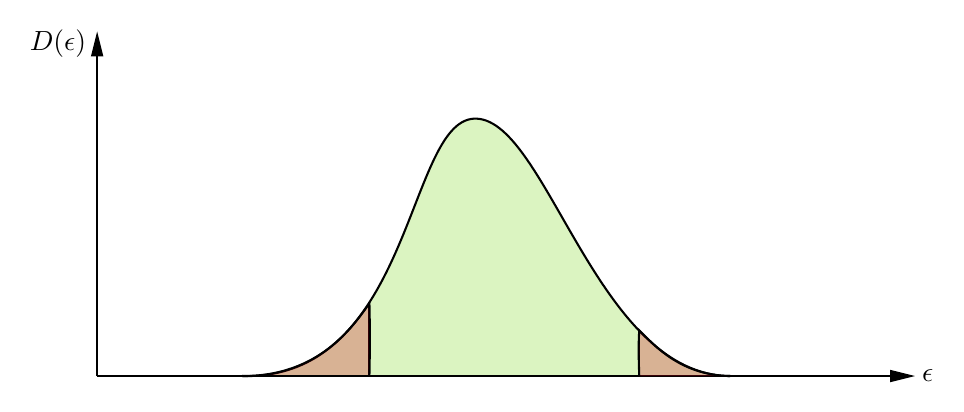
\begin{tikzpicture}[x=0.75pt,y=0.75pt,yscale=-1,xscale=1]
%uncomment if require: \path (0,300); %set diagram left start at 0, and has height of 300

%Curve Lines [id:da4027176161560928] 
\draw [fill={rgb, 255:red, 184; green, 233; blue, 134 }  ,fill opacity=0.51 ]   (155,186.17) .. controls (238,188.17) and (234,60.17) .. (268,62.17) .. controls (302,64.17) and (326.11,185.94) .. (390,186.17) ;
%Straight Lines [id:da13681751123326968] 
\draw    (85,186.17) -- (85,22.17) ;
\draw [shift={(85,20.17)}, rotate = 450] [fill={rgb, 255:red, 0; green, 0; blue, 0 }  ][line width=0.08]  [draw opacity=0] (12,-3) -- (0,0) -- (12,3) -- cycle    ;
%Straight Lines [id:da0169394948141961] 
\draw    (216.17,151.17) -- (216.17,186.17) ;
%Straight Lines [id:da6960384366783567] 
\draw    (346.17,164.17) -- (346.17,186.17) ;
%Curve Lines [id:da9091055633021599] 
\draw [fill={rgb, 255:red, 208; green, 2; blue, 27 }  ,fill opacity=0.27 ]   (155,186.17) .. controls (192,186.33) and (208.13,162.31) .. (216.17,151.17) .. controls (216.5,168.33) and (216.5,167.33) .. (216.17,186.17) ;
%Straight Lines [id:da6561575439712553] 
\draw    (85,186.17) -- (477,186.17) ;
\draw [shift={(479,186.17)}, rotate = 180] [fill={rgb, 255:red, 0; green, 0; blue, 0 }  ][line width=0.08]  [draw opacity=0] (12,-3) -- (0,0) -- (12,3) -- cycle    ;
%Curve Lines [id:da14298622888330836] 
\draw [fill={rgb, 255:red, 208; green, 2; blue, 27 }  ,fill opacity=0.27 ]   (346.17,186.17) .. controls (345.8,175.43) and (345.8,170.23) .. (346.17,164.17) .. controls (352.2,169.83) and (365,185.83) .. (390,186.17) ;

% Text Node
\draw (481,186.17) node [anchor=west] [inner sep=0.75pt]    {$\epsilon $};
% Text Node
\draw (81.21,26) node [anchor=east] [inner sep=0.75pt]    {$D( \epsilon )$};


\end{tikzpicture}
    \caption{一个无序系统的能带结构,延展态电子和局域态电子分别使用绿色和红色表示,两者的界限即为迁移率边}
    \label{fig:disorder-band}
\end{figure}

一些简单的论证可以说明这种模型的电子结构。
局域态和(能够长距离移动,从而能够导电的)延展态应该不共享能量。否则,设一个局域态和一个延展态具有一样的能量,那么将这个局域态和延展态做线性组合,得到另一个延展态,也能具有一样的能量,因此最终我们会发现,同一个能量上有一个被大量延展态环绕着的局域态,这种情况下我们其实可以直接忽略这个局域态。
$W=0$时我们有一个连续的延展态能带。通过微扰论可以发现,在这个能带两端的波函数将转化为局域态。% TODO
因此含有无序的金属的电子能带结构包括一个延展态能带和位于延展态能带两边的所谓的\concept{带尾局域态}(见\autoref{fig:disorder-band})。随着$W/t$的增大,会有越来越多的延展态转化为局域态。

现在费米面的位置将决定系统的导电性。如果费米面的位置位于较低的局域态能带中,虽然此时有能带半填充,但是由于是局域态,系统是绝缘体。
在实空间中,这等价于电子都被束缚在杂质周围。
费米面进入延展态能带后,所有能够被占据的杂质轨道都被占据了,电子别无他法,必须有一部分是延展态的。
在实空间中,这就好像大水漫灌将小水坑都灌满而仍然有不少剩余的可以四处流动。
当费米面进入较高的局域态能带时,延展态能带被占满,系统又一次变成绝缘体。
在实空间中,这就好像水缸被填满了,只留下几个气泡,然而气泡被定域在一些点附近无法移动。
改变费米面高度,或者更加容易的,改变$W/t$,因而能够产生一个延展-局域相变,或者说是金属-绝缘体相变。
这个相变通常称为\concept{Anderson转变}。
$W/t$增大只会让带尾局域态越来越多,最后延展态完全消失,因此无论费米面一开始在哪里,$W/t$足够大时都会发现金属-绝缘体相变,这正是前面通过分析$W/t=0$和$W/t \to \infty$而得出的结论。

\subsection{弱局域化}

上一节并没有解释为何当无序越来越强时到底发生了什么才导致局域化。本节将提供一些物理图像。

\subsubsection{单杂质下格林函数的微扰计算}

\eqref{eq:tight-binding-with-disorder}是自由理论,因此是严格可解的。通常我们会计算所谓的无序平均,即对每个可能的$\{\epsilon_{\vb*{i}}\}$构型,计算出某个物理量$O$(此处不是指可观察量算符,而是真的实行观测测得的量,如$\epsilon$给定后,某算符的期望值、方差,格林函数等),然后求出平均值$\overline{O}$。
对一个热力学系统,如果$O$是关于系统全局的,则$O$和无序平均$\overline{O}$大概率是非常接近的,这是等概率原理的空间版本。

我们要计算两点格林函数。两点关联函数为
\begin{equation}
    G^{-1}_{\vb*{i} \vb*{j}}(\ii \omega_n) = \omega_n + t_{\vb*{i} \vb*{j}} - \epsilon_{\vb*{i}} \delta_{\vb*{i} \vb*{j}}.
\end{equation}
这里我们去掉了松原格林函数前面的负号,以便于书写。
我们现在对$\epsilon_{\vb*{i}}$做微扰展开(虽然是自由系统但微扰展开总是合法的),就有
\begin{equation}
    \begin{aligned}
        G_{\vb*{i} \vb*{j}}(\ii \omega_n) &= \frac{1}{\ii \omega_n + t_{\vb*{i} \vb*{j}}} + \frac{1}{\ii \omega_n + t_{\vb*{i} \vb*{k}}} (- \epsilon_{\vb*{k}} \delta_{\vb*{k} \vb*{l}}) \frac{1}{\ii \omega_n + t_{\vb*{l} \vb*{j}}} + \cdots \\
        &= \frac{1}{\ii \omega_n - \hat{T}} + \frac{1}{\ii \omega_n - \hat{T}} \hat{\epsilon} \frac{1}{\ii \omega_n - \hat{T}} + \cdots,
    \end{aligned}
    \label{eq:disorder-scattered-fermion-green}
\end{equation}
这里我们已经引入了动能算符$\hat{T}$和微扰$\hat{\epsilon}$。
当然,这是非常直观的:电子和杂质散射了一次,两次,……
用格林函数计算出各种可以观测的物理量,对$\{\epsilon_{\vb*{i}}\}$求平均即可。%
\eqref{eq:disorder-scattered-fermion-green}的第一项在杂质构型平均中保留,第二项消失,因为出现了奇数个$\hat{\epsilon}$,第三项保留,为
\begin{equation}
    \overline{\frac{1}{\ii \omega_n - \hat{T}} \hat{\epsilon} \frac{1}{\ii \omega_n - \hat{T}} \hat{\epsilon} \frac{1}{\ii \omega_n - \hat{T}}} = \sum_{\vb*{j}} W^2 \frac{1}{\ii \omega_n - t_{\vb*{i} \vb*{j}}} \frac{1}{\ii \omega_n - t_{\vb*{j} \vb*{j}}} \frac{1}{\ii \omega_n - t_{\vb*{j} \vb*{k}} }.
    \label{eq:impurity-three-propagator-example}
\end{equation}
这里,两个$\hat{\epsilon}$同时出现,对它们求无序平均后就得到上式右边。
考虑更高阶项,如果不做杂质平均,得到的项就是链状的费曼图:
\[
    \begin{gathered}
        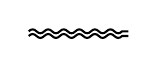
\begin{tikzpicture}[x=0.75pt,y=0.75pt,yscale=-0.75,xscale=0.75]
        %uncomment if require: \path (0,300); %set diagram left start at 0, and has height of 300

        %Straight Lines [id:da9866537023377491] 
        \draw    (138.71,172.98) .. controls (140.38,171.31) and (142.04,171.31) .. (143.71,172.98) .. controls (145.38,174.65) and (147.04,174.65) .. (148.71,172.98) .. controls (150.38,171.31) and (152.04,171.31) .. (153.71,172.98) .. controls (155.38,174.65) and (157.04,174.65) .. (158.71,172.98) .. controls (160.38,171.31) and (162.04,171.31) .. (163.71,172.98) .. controls (165.38,174.65) and (167.04,174.65) .. (168.71,172.98) .. controls (170.38,171.31) and (172.04,171.31) .. (173.71,172.98) .. controls (175.38,174.65) and (177.04,174.65) .. (178.71,172.98) .. controls (180.38,171.31) and (182.04,171.31) .. (183.71,172.98) .. controls (185.38,174.65) and (187.04,174.65) .. (188.71,172.98) .. controls (190.38,171.31) and (192.04,171.31) .. (193.71,172.98) .. controls (195.38,174.65) and (197.04,174.65) .. (198.71,172.98) -- (202.71,172.98) -- (202.71,172.98)(138.71,175.98) .. controls (140.38,174.31) and (142.04,174.31) .. (143.71,175.98) .. controls (145.38,177.65) and (147.04,177.65) .. (148.71,175.98) .. controls (150.38,174.31) and (152.04,174.31) .. (153.71,175.98) .. controls (155.38,177.65) and (157.04,177.65) .. (158.71,175.98) .. controls (160.38,174.31) and (162.04,174.31) .. (163.71,175.98) .. controls (165.38,177.65) and (167.04,177.65) .. (168.71,175.98) .. controls (170.38,174.31) and (172.04,174.31) .. (173.71,175.98) .. controls (175.38,177.65) and (177.04,177.65) .. (178.71,175.98) .. controls (180.38,174.31) and (182.04,174.31) .. (183.71,175.98) .. controls (185.38,177.65) and (187.04,177.65) .. (188.71,175.98) .. controls (190.38,174.31) and (192.04,174.31) .. (193.71,175.98) .. controls (195.38,177.65) and (197.04,177.65) .. (198.71,175.98) -- (202.71,175.98) -- (202.71,175.98) ;
        \end{tikzpicture}
    \end{gathered} = 
    \begin{gathered}
        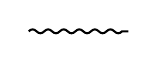
\begin{tikzpicture}[x=0.75pt,y=0.75pt,yscale=-0.75,xscale=0.75]
            %uncomment if require: \path (0,300); %set diagram left start at 0, and has height of 300
            
            %Straight Lines [id:da9866537023377491] 
            \draw    (138.71,174.48) .. controls (140.38,172.81) and (142.04,172.81) .. (143.71,174.48) .. controls (145.38,176.15) and (147.04,176.15) .. (148.71,174.48) .. controls (150.38,172.81) and (152.04,172.81) .. (153.71,174.48) .. controls (155.38,176.15) and (157.04,176.15) .. (158.71,174.48) .. controls (160.38,172.81) and (162.04,172.81) .. (163.71,174.48) .. controls (165.38,176.15) and (167.04,176.15) .. (168.71,174.48) .. controls (170.38,172.81) and (172.04,172.81) .. (173.71,174.48) .. controls (175.38,176.15) and (177.04,176.15) .. (178.71,174.48) .. controls (180.38,172.81) and (182.04,172.81) .. (183.71,174.48) .. controls (185.38,176.15) and (187.04,176.15) .. (188.71,174.48) .. controls (190.38,172.81) and (192.04,172.81) .. (193.71,174.48) .. controls (195.38,176.15) and (197.04,176.15) .. (198.71,174.48) -- (202.71,174.48) -- (202.71,174.48) ;
            \end{tikzpicture}            
    \end{gathered} 
    + \begin{gathered}
        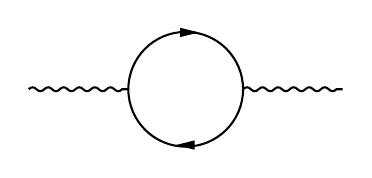
\begin{tikzpicture}[x=0.75pt,y=0.75pt,yscale=-0.75,xscale=0.75]
            %uncomment if require: \path (0,300); %set diagram left start at 0, and has height of 300
            
            %Straight Lines [id:da17567041601820987] 
            \draw    (118.71,154.48) .. controls (120.38,152.81) and (122.04,152.81) .. (123.71,154.48) .. controls (125.38,156.15) and (127.04,156.15) .. (128.71,154.48) .. controls (130.38,152.81) and (132.04,152.81) .. (133.71,154.48) .. controls (135.38,156.15) and (137.04,156.15) .. (138.71,154.48) .. controls (140.38,152.81) and (142.04,152.81) .. (143.71,154.48) .. controls (145.38,156.15) and (147.04,156.15) .. (148.71,154.48) .. controls (150.38,152.81) and (152.04,152.81) .. (153.71,154.48) .. controls (155.38,156.15) and (157.04,156.15) .. (158.71,154.48) .. controls (160.38,152.81) and (162.04,152.81) .. (163.71,154.48) .. controls (165.38,156.15) and (167.04,156.15) .. (168.71,154.48) .. controls (170.38,152.81) and (172.04,152.81) .. (173.71,154.48) .. controls (175.38,156.15) and (177.04,156.15) .. (178.71,154.48) -- (182.71,154.48) -- (182.71,154.48) ;
            %Shape: Circle [id:dp17564496306640676] 
            \draw   (182.71,154.48) .. controls (182.71,134.13) and (199.21,117.63) .. (219.56,117.63) .. controls (239.91,117.63) and (256.41,134.13) .. (256.41,154.48) .. controls (256.41,174.84) and (239.91,191.34) .. (219.56,191.34) .. controls (199.21,191.34) and (182.71,174.84) .. (182.71,154.48) -- cycle ;
            %Straight Lines [id:da5121293561595781] 
            \draw    (256.41,154.48) .. controls (258.08,152.81) and (259.74,152.81) .. (261.41,154.48) .. controls (263.08,156.15) and (264.74,156.15) .. (266.41,154.48) .. controls (268.08,152.81) and (269.74,152.81) .. (271.41,154.48) .. controls (273.08,156.15) and (274.74,156.15) .. (276.41,154.48) .. controls (278.08,152.81) and (279.74,152.81) .. (281.41,154.48) .. controls (283.08,156.15) and (284.74,156.15) .. (286.41,154.48) .. controls (288.08,152.81) and (289.74,152.81) .. (291.41,154.48) .. controls (293.08,156.15) and (294.74,156.15) .. (296.41,154.48) .. controls (298.08,152.81) and (299.74,152.81) .. (301.41,154.48) .. controls (303.08,156.15) and (304.74,156.15) .. (306.41,154.48) .. controls (308.08,152.81) and (309.74,152.81) .. (311.41,154.48) .. controls (313.08,156.15) and (314.74,156.15) .. (316.41,154.48) -- (320.41,154.48) -- (320.41,154.48) ;
            %Straight Lines [id:da4288732800639541] 
            \draw    (228,118) ;
            \draw [shift={(228,118)}, rotate = 180] [fill={rgb, 255:red, 0; green, 0; blue, 0 }  ][line width=0.08]  [draw opacity=0] (12,-3) -- (0,0) -- (12,3) -- cycle    ;
            %Straight Lines [id:da6676893206799264] 
            \draw    (220.56,190.34) -- (215.26,190.34) ;
            \draw [shift={(213.26,190.34)}, rotate = 360] [fill={rgb, 255:red, 0; green, 0; blue, 0 }  ][line width=0.08]  [draw opacity=0] (12,-3) -- (0,0) -- (12,3) -- cycle    ;
            \end{tikzpicture}                       
    \end{gathered}
    + \begin{gathered}
        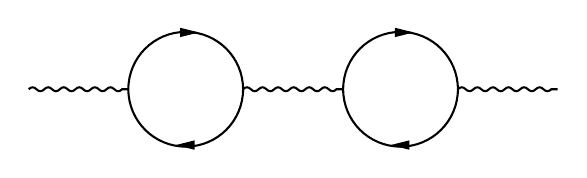
\begin{tikzpicture}[x=0.75pt,y=0.75pt,yscale=-0.75,xscale=0.75]
            %uncomment if require: \path (0,300); %set diagram left start at 0, and has height of 300
            
            %Straight Lines [id:da04781449358470047] 
            \draw    (138.71,174.48) .. controls (140.38,172.81) and (142.04,172.81) .. (143.71,174.48) .. controls (145.38,176.15) and (147.04,176.15) .. (148.71,174.48) .. controls (150.38,172.81) and (152.04,172.81) .. (153.71,174.48) .. controls (155.38,176.15) and (157.04,176.15) .. (158.71,174.48) .. controls (160.38,172.81) and (162.04,172.81) .. (163.71,174.48) .. controls (165.38,176.15) and (167.04,176.15) .. (168.71,174.48) .. controls (170.38,172.81) and (172.04,172.81) .. (173.71,174.48) .. controls (175.38,176.15) and (177.04,176.15) .. (178.71,174.48) .. controls (180.38,172.81) and (182.04,172.81) .. (183.71,174.48) .. controls (185.38,176.15) and (187.04,176.15) .. (188.71,174.48) .. controls (190.38,172.81) and (192.04,172.81) .. (193.71,174.48) .. controls (195.38,176.15) and (197.04,176.15) .. (198.71,174.48) -- (202.71,174.48) -- (202.71,174.48) ;
            %Shape: Circle [id:dp5727624261999054] 
            \draw   (202.71,174.48) .. controls (202.71,154.13) and (219.21,137.63) .. (239.56,137.63) .. controls (259.91,137.63) and (276.41,154.13) .. (276.41,174.48) .. controls (276.41,194.84) and (259.91,211.34) .. (239.56,211.34) .. controls (219.21,211.34) and (202.71,194.84) .. (202.71,174.48) -- cycle ;
            %Straight Lines [id:da22747154750459764] 
            \draw    (276.41,174.48) .. controls (278.08,172.81) and (279.74,172.81) .. (281.41,174.48) .. controls (283.08,176.15) and (284.74,176.15) .. (286.41,174.48) .. controls (288.08,172.81) and (289.74,172.81) .. (291.41,174.48) .. controls (293.08,176.15) and (294.74,176.15) .. (296.41,174.48) .. controls (298.08,172.81) and (299.74,172.81) .. (301.41,174.48) .. controls (303.08,176.15) and (304.74,176.15) .. (306.41,174.48) .. controls (308.08,172.81) and (309.74,172.81) .. (311.41,174.48) .. controls (313.08,176.15) and (314.74,176.15) .. (316.41,174.48) .. controls (318.08,172.81) and (319.74,172.81) .. (321.41,174.48) .. controls (323.08,176.15) and (324.74,176.15) .. (326.41,174.48) .. controls (328.08,172.81) and (329.74,172.81) .. (331.41,174.48) .. controls (333.08,176.15) and (334.74,176.15) .. (336.41,174.48) -- (340.41,174.48) -- (340.41,174.48) ;
            %Straight Lines [id:da1227681301369512] 
            \draw    (248,138) ;
            \draw [shift={(248,138)}, rotate = 180] [fill={rgb, 255:red, 0; green, 0; blue, 0 }  ][line width=0.08]  [draw opacity=0] (12,-3) -- (0,0) -- (12,3) -- cycle    ;
            %Straight Lines [id:da6960046996744582] 
            \draw    (240.56,210.34) -- (235.26,210.34) ;
            \draw [shift={(233.26,210.34)}, rotate = 360] [fill={rgb, 255:red, 0; green, 0; blue, 0 }  ][line width=0.08]  [draw opacity=0] (12,-3) -- (0,0) -- (12,3) -- cycle    ;
            %Shape: Circle [id:dp9324982228573173] 
            \draw   (340.71,174.48) .. controls (340.71,154.13) and (357.21,137.63) .. (377.56,137.63) .. controls (397.91,137.63) and (414.41,154.13) .. (414.41,174.48) .. controls (414.41,194.84) and (397.91,211.34) .. (377.56,211.34) .. controls (357.21,211.34) and (340.71,194.84) .. (340.71,174.48) -- cycle ;
            %Straight Lines [id:da5761762164736703] 
            \draw    (414.41,174.48) .. controls (416.08,172.81) and (417.74,172.81) .. (419.41,174.48) .. controls (421.08,176.15) and (422.74,176.15) .. (424.41,174.48) .. controls (426.08,172.81) and (427.74,172.81) .. (429.41,174.48) .. controls (431.08,176.15) and (432.74,176.15) .. (434.41,174.48) .. controls (436.08,172.81) and (437.74,172.81) .. (439.41,174.48) .. controls (441.08,176.15) and (442.74,176.15) .. (444.41,174.48) .. controls (446.08,172.81) and (447.74,172.81) .. (449.41,174.48) .. controls (451.08,176.15) and (452.74,176.15) .. (454.41,174.48) .. controls (456.08,172.81) and (457.74,172.81) .. (459.41,174.48) .. controls (461.08,176.15) and (462.74,176.15) .. (464.41,174.48) .. controls (466.08,172.81) and (467.74,172.81) .. (469.41,174.48) .. controls (471.08,176.15) and (472.74,176.15) .. (474.41,174.48) -- (478.41,174.48) -- (478.41,174.48) ;
            %Straight Lines [id:da712226604774016] 
            \draw    (386,138) ;
            \draw [shift={(386,138)}, rotate = 180] [fill={rgb, 255:red, 0; green, 0; blue, 0 }  ][line width=0.08]  [draw opacity=0] (12,-3) -- (0,0) -- (12,3) -- cycle    ;
            %Straight Lines [id:da3541004059124153] 
            \draw    (378.56,210.34) -- (373.26,210.34) ;
            \draw [shift={(371.26,210.34)}, rotate = 360] [fill={rgb, 255:red, 0; green, 0; blue, 0 }  ][line width=0.08]  [draw opacity=0] (12,-3) -- (0,0) -- (12,3) -- cycle    ;
            \end{tikzpicture}                
    \end{gathered} + \cdots,
\]
由于杂质分布取高斯分布,Wick定理对杂质平均同样适用,因此将量子力学微扰论的每一项做杂质分布,图形地说就是将上图中的叉($\epsilon_i c^\dagger_i c_i$项的微扰)两两配对,并引入“相互作用”顶角(整个理论实际上当然还是自由的,并无真正的相互作用,但是$W^2$确实构成微扰)
\begin{equation}
    \begin{gathered}
        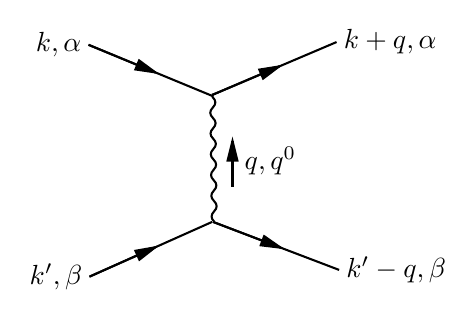
\begin{tikzpicture}[x=0.75pt,y=0.75pt,yscale=-1,xscale=1]
            %Straight Lines [id:da15915538235750892] 
            \draw    (100.17,172.51) -- (131.95,158.32) ;
            \draw [shift={(133.77,157.5)}, rotate = 515.9300000000001] [fill={rgb, 255:red, 0; green, 0; blue, 0 }  ][line width=0.08]  [draw opacity=0] (12,-3) -- (0,0) -- (12,3) -- cycle    ;
            %Straight Lines [id:da595892295722313] 
            \draw    (100.17,172.51) -- (159.26,146.12) ;
            
            %Straight Lines [id:da41375516068648066] 
            \draw    (160.29,146.04) .. controls (158.6,144.39) and (158.57,142.73) .. (160.22,141.04) .. controls (161.87,139.35) and (161.85,137.69) .. (160.16,136.04) .. controls (158.47,134.39) and (158.45,132.73) .. (160.1,131.04) .. controls (161.74,129.35) and (161.72,127.69) .. (160.03,126.04) .. controls (158.34,124.39) and (158.32,122.73) .. (159.97,121.04) .. controls (161.62,119.35) and (161.6,117.69) .. (159.91,116.04) .. controls (158.22,114.39) and (158.2,112.73) .. (159.84,111.04) .. controls (161.49,109.35) and (161.47,107.69) .. (159.78,106.04) .. controls (158.09,104.39) and (158.07,102.73) .. (159.72,101.04) .. controls (161.36,99.35) and (161.34,97.69) .. (159.65,96.04) .. controls (157.96,94.39) and (157.94,92.73) .. (159.59,91.04) .. controls (161.24,89.35) and (161.22,87.69) .. (159.53,86.04) -- (159.51,84.35) -- (159.51,84.35) ;
            %Straight Lines [id:da18427908684914152] 
            \draw    (159.7,146.12) -- (192.38,158.57) ;
            \draw [shift={(194.25,159.28)}, rotate = 200.85] [fill={rgb, 255:red, 0; green, 0; blue, 0 }  ][line width=0.08]  [draw opacity=0] (12,-3) -- (0,0) -- (12,3) -- cycle    ;
            %Straight Lines [id:da5517253733622631] 
            \draw    (159.7,146.12) -- (220.46,169.26) ;
            
            %Straight Lines [id:da9982758254698763] 
            \draw    (99.72,60.8) -- (131.97,74.12) ;
            \draw [shift={(133.82,74.88)}, rotate = 202.44] [fill={rgb, 255:red, 0; green, 0; blue, 0 }  ][line width=0.08]  [draw opacity=0] (12,-3) -- (0,0) -- (12,3) -- cycle    ;
            %Straight Lines [id:da26812450354509565] 
            \draw    (99.72,60.8) -- (159.69,85.57) ;
            
            %Straight Lines [id:da1756933542309722] 
            \draw    (159.57,84.84) -- (191.65,71.2) ;
            \draw [shift={(193.49,70.41)}, rotate = 516.96] [fill={rgb, 255:red, 0; green, 0; blue, 0 }  ][line width=0.08]  [draw opacity=0] (12,-3) -- (0,0) -- (12,3) -- cycle    ;
            %Straight Lines [id:da7638586957076614] 
            \draw    (159.57,84.84) -- (219.22,59.47) ;
            
            %Straight Lines [id:da9798265876333652] 
            \draw    (169.09,129.1) -- (169.09,107.04) ;
            \draw [shift={(169.09,105.04)}, rotate = 450] [fill={rgb, 255:red, 0; green, 0; blue, 0 }  ][line width=0.08]  [draw opacity=0] (12,-3) -- (0,0) -- (12,3) -- cycle    ;
            
            % Text Node
            \draw (97.72,60.8) node [anchor=east] [inner sep=0.75pt]    {$\boldsymbol{k} ,\alpha $};
            % Text Node
            \draw (221.22,59.47) node [anchor=west] [inner sep=0.75pt]    {$\boldsymbol{k} +\boldsymbol{q} ,\alpha $};
            % Text Node
            \draw (173.48,108.5) node [anchor=north west][inner sep=0.75pt]    {$\boldsymbol{q}, \ii q^0$};
            % Text Node
            \draw (98.17,172.51) node [anchor=east] [inner sep=0.75pt]    {$\boldsymbol{k} ',\beta $};
            % Text Node
            \draw (222.46,169.26) node [anchor=west] [inner sep=0.75pt]    {$\boldsymbol{k} '-\boldsymbol{q} ,\beta $};
            \end{tikzpicture}
    \end{gathered} = \frac{1}{V} \frac{4\pi e^2}{\abs*{\vb*{q}}^2},
\end{equation}
直观地看,这是说电子运动路径如果经过它曾经经过的某一点,那么这个路径的权重就很大。
这样\eqref{eq:impurity-three-propagator-example}可以直观地写成
\begin{equation}
    \begin{gathered}
        \begin{tikzpicture}[x=0.75pt,y=0.75pt,yscale=-0.75,xscale=0.75]
            %uncomment if require: \path (0,300); %set diagram left start at 0, and has height of 300
            
            %Straight Lines [id:da5173414445626214] 
            \draw    (107,177) -- (194.71,177) ;
            \draw [shift={(150.85,177)}, rotate = 180] [fill={rgb, 255:red, 0; green, 0; blue, 0 }  ][line width=0.08]  [draw opacity=0] (12,-3) -- (0,0) -- (12,3) -- cycle    ;
            %Straight Lines [id:da47983403227869514] 
            \draw    (194.71,177) -- (282.41,177) ;
            \draw [shift={(238.56,177)}, rotate = 180] [fill={rgb, 255:red, 0; green, 0; blue, 0 }  ][line width=0.08]  [draw opacity=0] (12,-3) -- (0,0) -- (12,3) -- cycle    ;
            %Straight Lines [id:da2596488833001649] 
            \draw    (282.41,177) -- (370.12,177) ;
            \draw [shift={(326.26,177)}, rotate = 180] [fill={rgb, 255:red, 0; green, 0; blue, 0 }  ][line width=0.08]  [draw opacity=0] (12,-3) -- (0,0) -- (12,3) -- cycle    ;
            %Straight Lines [id:da902407644674809] 
            \draw  [dash pattern={on 4.5pt off 4.5pt}]  (194.71,177) -- (236.71,98.9) ;
            %Straight Lines [id:da7883885352481057] 
            \draw  [dash pattern={on 4.5pt off 4.5pt}]  (236.71,98.9) -- (282.41,177) ;
            
            % Text Node
            \draw (107,180.4) node [anchor=north] [inner sep=0.75pt]    {$\boldsymbol{i}$};
            % Text Node
            \draw (194.71,180.4) node [anchor=north] [inner sep=0.75pt]    {$\boldsymbol{j}$};
            % Text Node
            \draw (370.12,180.4) node [anchor=north] [inner sep=0.75pt]    {$\boldsymbol{k}$};
            % Text Node
            \draw (282.41,180.4) node [anchor=north] [inner sep=0.75pt]    {$\boldsymbol{j} '$};
            \end{tikzpicture}            
    \end{gathered} = W^2 \delta_{\vb*{j} \vb*{j}'} \frac{1}{\ii \omega_n - t_{\vb*{i} \vb*{j}}} \frac{1}{\ii \omega_n - t_{\vb*{j} \vb*{j}}} \frac{1}{\ii \omega_n - t_{\vb*{j}' \vb*{k}} }.
\end{equation}
我们也可以定义动量空间中的费曼规则。计算两点关联函数的二阶微扰$G^{(2)}_{\vb*{i} \vb*{k}}$的傅里叶变换,有
\[
    \begin{aligned}
        G^{(2)}(\vb*{k}, \ii \omega_n) &= \frac{1}{N} \sum_{\vb*{i}, \vb*{l}} \ee^{- \ii \vb*{k} \cdot (\vb*{R}_{\vb*{i}} - \vb*{R}_{\vb*{l}})} \sum_{\vb*{j}} G_{\vb*{i} \vb*{j}}^{0} G_{\vb*{j} \vb*{j}}^{0} G_{\vb*{j} \vb*{l}}^0 W^2 \\
        &= \frac{1}{N} W^2 \sum_{\vb*{k}'} G_{\vb*{k}}^0 G_{\vb*{k}'}^0 G_{\vb*{k}}^0,
    \end{aligned}
\]
第一行的$1/N$因子是我们同时对$\vb*{i}$和$\vb*{j}$求和所致;第二个等号来自
\[
    G_{\vb*{j} \vb*{j}}^0 = \frac{1}{N} \sum_{\vb*{k}} G^{0}_{\vb*{k}}.
\]
因此动量空间的顶角就是
\begin{equation}
    \begin{gathered}
        \begin{tikzpicture}[x=0.75pt,y=0.75pt,yscale=-1,xscale=1]
            %uncomment if require: \path (0,300); %set diagram left start at 0, and has height of 300
            
            %Shape: Arc [id:dp038937042441603786] 
            \draw  [draw opacity=0][dash pattern={on 4.5pt off 4.5pt}] (234.71,216.74) .. controls (234.7,216.48) and (234.7,216.21) .. (234.7,215.94) .. controls (234.6,192.83) and (253.81,174.02) .. (277.61,173.92) .. controls (301.41,173.82) and (320.78,192.47) .. (320.88,215.58) .. controls (320.88,215.95) and (320.88,216.33) .. (320.87,216.7) -- (277.79,215.76) -- cycle ; \draw  [dash pattern={on 4.5pt off 4.5pt}] (234.71,216.74) .. controls (234.7,216.48) and (234.7,216.21) .. (234.7,215.94) .. controls (234.6,192.83) and (253.81,174.02) .. (277.61,173.92) .. controls (301.41,173.82) and (320.78,192.47) .. (320.88,215.58) .. controls (320.88,215.95) and (320.88,216.33) .. (320.87,216.7) ;
            %Straight Lines [id:da6230366533912561] 
            \draw    (309.02,216.7) -- (332.72,216.7) ;
            %Straight Lines [id:da48571072364504575] 
            \draw    (222.85,216.74) -- (246.56,216.74) ;
            
            % Text Node
            \draw (234.71,220.14) node [anchor=north] [inner sep=0.75pt]    {$\boldsymbol{k}$};
            % Text Node
            \draw (320.87,220.1) node [anchor=north] [inner sep=0.75pt]    {$\boldsymbol{k}'$};
            \end{tikzpicture}            
    \end{gathered} = \frac{1}{N} W^2 \delta_{\vb*{k} \vb*{k}'}.
    \label{eq:disorder-mom-space-vertex}
\end{equation}
可以看到该顶角函数要求入射、出射动量守恒,但是并不保证$\vb*{k}$顶点和$\vb*{k}'$顶点之间的传播子动量守恒。
这是意料之中的,因为坐标空间中的费曼规则要求某两次散射发生在同一个地点,这个地点上的动量守恒条件实际上就是出入动量相等,但是不保证“内部”的动量和出入动量完全一样。
虽然杂质破缺了空间平移对称性,但是因为杂质平均后空间平移对称性仍然成立,某种动量守恒还是成立的。
此外也可以注意到,\eqref{eq:disorder-mom-space-vertex}中有一个因子$1/N$,虽然杂质造成的微扰只含有两个场算符,按理说切换到动量空间后不应该有任何含有$N$的因子;然而由于\eqref{eq:disorder-mom-space-vertex}实际上是\emph{两个}$\hat{\epsilon}$乘在一起求平均的结果,它等效地相当于一个\emph{二粒子相互作用顶角},因此有因子$1/N$是不奇怪的。
于是动量空间中的\eqref{eq:impurity-three-propagator-example}就是
\begin{equation}
    \begin{gathered}
        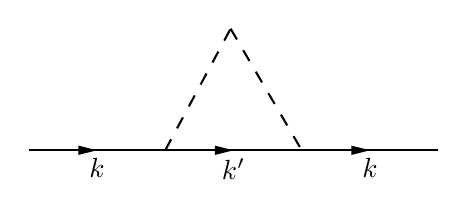
\begin{tikzpicture}[x=0.75pt,y=0.75pt,yscale=-0.75,xscale=0.75]
            %uncomment if require: \path (0,300); %set diagram left start at 0, and has height of 300
            
            %Straight Lines [id:da442216852880003] 
            \draw    (127,197) -- (214.71,197) ;
            \draw [shift={(170.85,197)}, rotate = 180] [fill={rgb, 255:red, 0; green, 0; blue, 0 }  ][line width=0.08]  [draw opacity=0] (12,-3) -- (0,0) -- (12,3) -- cycle    ;
            %Straight Lines [id:da6609253169175426] 
            \draw    (214.71,197) -- (302.41,197) ;
            \draw [shift={(258.56,197)}, rotate = 180] [fill={rgb, 255:red, 0; green, 0; blue, 0 }  ][line width=0.08]  [draw opacity=0] (12,-3) -- (0,0) -- (12,3) -- cycle    ;
            %Straight Lines [id:da09219286573152496] 
            \draw    (302.41,197) -- (390.12,197) ;
            \draw [shift={(346.26,197)}, rotate = 180] [fill={rgb, 255:red, 0; green, 0; blue, 0 }  ][line width=0.08]  [draw opacity=0] (12,-3) -- (0,0) -- (12,3) -- cycle    ;
            %Straight Lines [id:da6927930190889249] 
            \draw  [dash pattern={on 4.5pt off 4.5pt}]  (214.71,197) -- (256.71,118.9) ;
            %Straight Lines [id:da14008540153714755] 
            \draw  [dash pattern={on 4.5pt off 4.5pt}]  (256.71,118.9) -- (302.41,197) ;
            
            % Text Node
            \draw (170.85,200.4) node [anchor=north] [inner sep=0.75pt]    {$\boldsymbol{k}$};
            % Text Node
            \draw (346.26,200.4) node [anchor=north] [inner sep=0.75pt]    {$\boldsymbol{k}$};
            % Text Node
            \draw (258.56,200.4) node [anchor=north] [inner sep=0.75pt]    {$\boldsymbol{k} '$};
            \end{tikzpicture}            
    \end{gathered} = \frac{1}{N} W^2 \sum_{\vb*{k}'} G_{\vb*{k}}^0 G_{\vb*{k}'}^0 G_{\vb*{k}}^0.
\end{equation}
将无穷多个图加在一起实际上给出的就是自能修正。“一圈图”(虽然实际上是树图,因为虚线不提供传播子,也就没有圈图积分)的自能修正是
\begin{equation}
    \overline{G(\vb*{k}, \ii \omega_n)} = \frac{1}{\ii \omega_n - \xi_{\vb*{k}} - \Sigma}  ,
\end{equation}
其中自能就是
\begin{equation}
    \Sigma = W^2 \frac{1}{N} \sum_{\vb*{k}'} \frac{1}{\ii \omega_n - \xi_{\vb*{k}'}}
\end{equation}
或者换成推迟格林函数中的自能,是
\begin{equation}
    \overline{G^\text{ret}(\vb*{k}, \omega)} = \frac{1}{\omega - \xi_{\vb*{k}} - \Sigma + \ii 0^+} , \quad \Sigma^\text{ret} = W^2 \frac{1}{N} \sum_{\vb*{k}'} \frac{1}{\omega - \xi_{\vb*{k}'}  + \ii 0^+}.
\end{equation}
这个自能修正的实部是非常平凡的,除了平移了一下化学势以外什么也没有做,而其虚部
\begin{equation}
    \Im \Sigma^\text{ret} = - \pi W^2 \frac{1}{N} \sum_{\vb*{k}'} \delta(\omega - \xi_{\vb*{k}'}) = - \pi W^2 V_\text{u.c.} N(0).
\end{equation}
则给出了电子的寿命,实际上最好说是电子的动量模式的寿命,即电子运动着运动着就被散射到别的动量模式上了。通过计算电子寿命可以得到体系的电阻。

\subsubsection{随机游走图像}

系统中总是有大量热涨落,因此电子在长距离运动时会出现退相干。
设$l$为电子的相干长度,则参数
\begin{equation}
    \gamma = \frac{1}{\pi k_\text{F} l}
\end{equation}
表征了长距离相干性。在$\gamma$非常小时,两个杂质的间距远大于电子相关长度,因此可以使用经典模型处理问题。
这样,我们认为电子以费米速度运动,并与杂质发生弹性碰撞。于是可以认为电子在做一个随机行走,两步之间没有任何关联。
这是一个完全经典的过程,两条路径之间没有任何干涉。
实际上这就是Drude模型。因此,在纯粹经典的情况下,杂质增多会缩短电子的平均自由程,但是它只会让电子线性上升,不会让系统一下子变成绝缘体。

现在假定虽然$\gamma$很小,但相干的散射还是可能的。这样两点之间的跃迁概率就会出现超越经典模型的修正。
从一个点出发经过一系列点然后又回来的路径会因为相干叠加而获得更大的概率(经典概率的两倍)。
这正是我们在费曼图计算中看到的:$W$项的引入会导致\eqref{eq:disorder-real-space-vertex},它要求电子运动经过它曾经经过的某一点。
从电子的能量本征态的角度,这意味着在杂质数量较多时将会形成电子在几个杂质之间打转的模式。
这种模式的电子是不能够导电的,因为它是局域态而不是延展态。

电子运动情况的空间系综平均等价于一个随机行走
\[
    \expval*{r^2}(t) = D_0 t = \frac{l^2}{\tau} t = v_\text{F}^2 \tau t.
\]
在时间$t$内,电子经典情况下可以到达的体积为
\[
    V(t) \sim (\sqrt{D_0 t})^d = (D_0 t)^{d/2},
\]
如果其体积在一个大小为
\[
    \sim \lambda_\text{F}^{d-1} v_\text{F} \dd{t}
\]
的圆柱体中,那么在$t$到$t+\dd{t}$时间内它就可以回到原点。这样
\[
    P_{a \to a} \sim \int \frac{\lambda_\text{F}^{d-1} v_\text{F} \dd{t}}{(D_0 t)^{d/2}} 
\]
积分下限的数量级为$\tau$,因为在比这更小的时间尺度上,电子的运动只是布朗运动,不是较连续的扩散。
积分上限为退相干时间$\tau_\phi$,它也许来自电子和热化的声子的相互作用或是电子电子相互作用,无论如何都涉及一些有限温的机制。
\[
    \frac{\var{\sigma}}{\sigma_0} = - \lambda_\text{d} \begin{cases}
        \sqrt{\frac{\tau_\phi}{\tau}}, \quad &d = 1, \\
        \ln(\frac{\tau_\phi}{\tau}) , \quad &d = 2, \\
        \sqrt{\frac{\tau}{\tau_\phi}} , \quad &d = 3.
    \end{cases}
\]
当$T\to 0$时,$d=1, 2$的情况给出了缺乏物理意义的结果:电导率趋向负无穷。这意味着此时微扰论失效。
物理地分析,此时所有电子能量本征态都只可能是局域态,因此电导率为零,系统变为绝缘体。
$d=3$时随着温度降低,电导降至零,因此同样系统变为了绝缘体。

\subsection{Thouless论证和重整化群}

由于$d=1, 2$的情况是超越微扰论的,需要使用重整化群的理论来分析问题。
记归一化无量纲电导为
\begin{equation}
    g = \frac{G}{e^2 / \hbar},
\end{equation}
其中$G$为电导,它和材料的长度尺度$L$有关。将$L$看成重整化群参数,$L$增大表示往宏观性质方向移动。
这样$\beta$函数定义为
\begin{equation}
    \beta(g(L)) = \dv{\ln g}{\ln L}.    
\end{equation}

对$g \gg 1$的情况,即良导体极限,由电阻定律
\[
    g = \sigma / (e^2 / \hbar) L^{d-2},
\]
则
\[
    \beta(g) = d - 2.
\]
实际上,无序的存在会让电阻变大,电导变小,即会让$\ln g$增长得没有那么快,于是对$g$比较大的情况,我们做一阶展开:
\begin{equation}
    \beta(g) = d - 2 - c \frac{1}{g},
    \label{eq:disorder-rg-large-g}
\end{equation}
其中$c$是一个大于零的常数。

对$g \ll 1$的情况即绝缘体的情况,电导会随着系统尺度快速衰减,通常是指数衰减:
\[
    g = g_0 \ee^{- L / \xi},
\]
于是
\begin{equation}
    \beta(g) = \ln(\frac{g}{g_0}).
    \label{eq:disorder-rg-small-g}
\end{equation}
实际的$\beta$函数应该在\eqref{eq:disorder-rg-large-g}和\eqref{eq:disorder-rg-small-g}之间。
绘图可知,对$d=1, 2$的情况,$\beta$函数始终小于零,因此在$L$增大时$g$会衰减到零。换而言之,这两个情况下含有无序的固体只有一个地能有效理论,就是完全的局域化。
三维系统的$\beta$函数有一个零点$g_\text{c}$,如果一开始$g < g_\text{c}$,那么$\beta$函数始终是负的,于是重整化之后$g=0$,得到一个绝缘体相;如果一开始$g > g_\text{c}$,那么$\beta$函数始终是正的,重整化之后得到一个导体相。
换而言之$g_\text{c}$是一个相变点。

对三维情况,在相变点附加将$\beta$函数线性化,有
\begin{equation}
    \beta(g) = s \left( \frac{g - g_\text{c}}{g_\text{c}} \right),
\end{equation}
计算得到
\begin{equation}
    \frac{g(L) - g_\text{c}}{g_\text{c}} = \left( \frac{L}{} \right)
\end{equation}
